\chapter{Systems of Particles, Variable Mass, and Collisions}
\label{ch:systems_collisions}

\begin{chapterintro}
\textbf{Chapter Objectives:} In this concluding theoretical chapter, we generalize point-mass mechanics to multi-particle systems and open thermodynamic systems of variable mass. You will master the Center of Mass theorem; prove Koenig's first and second theorems; derive the Meshchersky and Tsiolkovsky rocket equations; evaluate gravity losses and multi-stage launch vehicles; and calculate elastic and inelastic collision kinematics in laboratory and center-of-mass frames.
\end{chapterintro}

\section{Center of Mass and Koenig's Theorems}

Consider an arbitrary system of $N$ discrete material points $\{M_i\}_{i=1}^N$, each possessing inertial mass $m_i$ and located at position vector $\vec{r}_i$ in an inertial frame $\mathcal{R}$.
The total mass of the system is:
\begin{equation}
M \eqdef \sum_{i=1}^N m_i.
\end{equation}

\begin{definitionbox}{Center of Mass (Barycenter)}
The \textbf{center of mass} $G$ of the system is the unique point defined by:
\begin{equation}
\vec{R}_G \eqdef \frac{1}{M} \sum_{i=1}^N m_i \vec{r}_i \iff \sum_{i=1}^N m_i \vec{GM_i} \equiv \vzero.
\end{equation}
The total linear momentum $\vec{P}$ of the system equals the momentum of a single hypothetical particle of mass $M$ moving with the velocity of the center of mass $\vec{v}_G = \dot{\vec{R}}_G$:
\begin{equation}
\vec{P} \eqdef \sum_{i=1}^N m_i \vec{v}_i = M \vec{v}_G.
\end{equation}
\end{definitionbox}

\subsection{The Center of Mass Theorem}

The net force acting on each particle $M_i$ consists of external forces $\vec{F}_i^{\text{ext}}$ exerted by bodies outside the system and internal interaction forces $\vec{F}_{j \to i}$ exerted by all other particles $j \neq i$ inside the system:
\[
m_i \frac{\dd\vec{v}_i}{\dd t} = \vec{F}_i^{\text{ext}} + \sum_{j \neq i}^N \vec{F}_{j \to i}.
\]
Summing over all $N$ particles:
\[
\frac{\dd\vec{P}}{\dd t} = \sum_{i=1}^N m_i \frac{\dd\vec{v}_i}{\dd t} = \sum_{i=1}^N \vec{F}_i^{\text{ext}} + \sum_{i=1}^N \sum_{j \neq i}^N \vec{F}_{j \to i}.
\]
According to Newton's third law of action and reaction, the internal pairwise forces are mutually equal and opposite: $\vec{F}_{j \to i} + \vec{F}_{i \to j} = \vzero$. Consequently, the double sum over all internal forces vanishes identically!

\begin{lawbox}{The Center of Mass Theorem}
The center of mass $G$ of any system of particles accelerates as if the total mass $M$ were concentrated at $G$ and acted upon by the resultant of all \textbf{external forces} alone:
\begin{equation}
\frac{\dd\vec{P}}{\dd t} = M \vec{a}_G = \vec{F}_{\text{ext}}^{\text{net}} = \sum_{i=1}^N \vec{F}_i^{\text{ext}}.
\end{equation}
\textbf{Law of Conservation of Total Momentum:} If the net external force on a system is zero ($\vec{F}_{\text{ext}}^{\text{net}} = \vzero$), the total linear momentum is strictly conserved:
\begin{equation}
\vec{P} = M \vec{v}_G = \text{constant vector}.
\end{equation}
The center of mass moves in uniform rectilinear motion regardless of any explosions, collisions, or internal chemical reactions taking place inside the system!
\end{lawbox}

\subsection{Koenig's Theorems for Energy and Angular Momentum}

Let $\mathcal{R}^*$ denote the \textbf{Center-of-Mass Frame} (barycentric frame), which translates with velocity $\vec{v}_G$ relative to $\mathcal{R}$ without rotation.
The relative positions and velocities in $\mathcal{R}^*$ are:
\begin{equation}
\vec{r}_i^* \eqdef \vec{r}_i - \vec{R}_G, \qquad \vec{v}_i^* \eqdef \vec{v}_i - \vec{v}_G.
\end{equation}
By definition of the center of mass, the total momentum in the barycentric frame is identically zero:
\begin{equation}
\vec{P}^* \eqdef \sum_{i=1}^N m_i \vec{v}_i^* = \sum_{i=1}^N m_i (\vec{v}_i - \vec{v}_G) = M \vec{v}_G - M \vec{v}_G \equiv \vzero.
\end{equation}

\begin{lawbox}{Koenig's First Theorem (Kinetic Energy)}
The total kinetic energy $E_k$ of a system of particles in frame $\mathcal{R}$ decomposes cleanly into the kinetic energy of the center of mass carrying the entire mass $M$, plus the internal kinetic energy $E_k^*$ evaluated in the center-of-mass frame:
\begin{equation}
E_k = \frac{1}{2} M v_G^2 + E_k^*, \qquad E_k^* \eqdef \frac{1}{2} \sum_{i=1}^N m_i (v_i^*)^2.
\end{equation}
\end{lawbox}

\paragraph{Proof.}
Expanding the kinetic energy sum:
\[
E_k = \frac{1}{2}\sum m_i (\vec{v}_G + \vec{v}_i^*)\cdot(\vec{v}_G + \vec{v}_i^*) = \frac{1}{2}\left(\sum m_i\right) v_G^2 + \vec{v}_G \cdot \underbrace{\left(\sum m_i \vec{v}_i^*\right)}_{= \vzero} + \frac{1}{2}\sum m_i (v_i^*)^2 = \frac{1}{2} M v_G^2 + E_k^*. \quad \blacksquare
\]

\begin{lawbox}{Koenig's Second Theorem (Angular Momentum)}
The total angular momentum $\vec{L}_O$ with respect to a fixed point $O$ equals the angular momentum of the center of mass about $O$, plus the internal angular momentum $\vec{L}^*$ about the center of mass:
\begin{equation}
\vec{L}_O = \vec{R}_G \times M \vec{v}_G + \vec{L}^*, \qquad \vec{L}^* \eqdef \sum_{i=1}^N \vec{r}_i^* \times m_i \vec{v}_i^*.
\end{equation}
\end{lawbox}

\section{Systems of Variable Mass and Rocket Propulsion}

Newton's second law $\vec{F} = \dd\vec{p}/\dd t$ cannot be directly written as $\vec{F} = \frac{\dd(m\vec{v})}{\dd t} = m\dot{\vec{v}} + \dot{m}\vec{v}$ for open systems where mass crosses the system boundary. We must rigorously track the momentum flux.

\begin{figure}[htbp]
\centering
\begin{minipage}{0.48\textwidth}
\centering
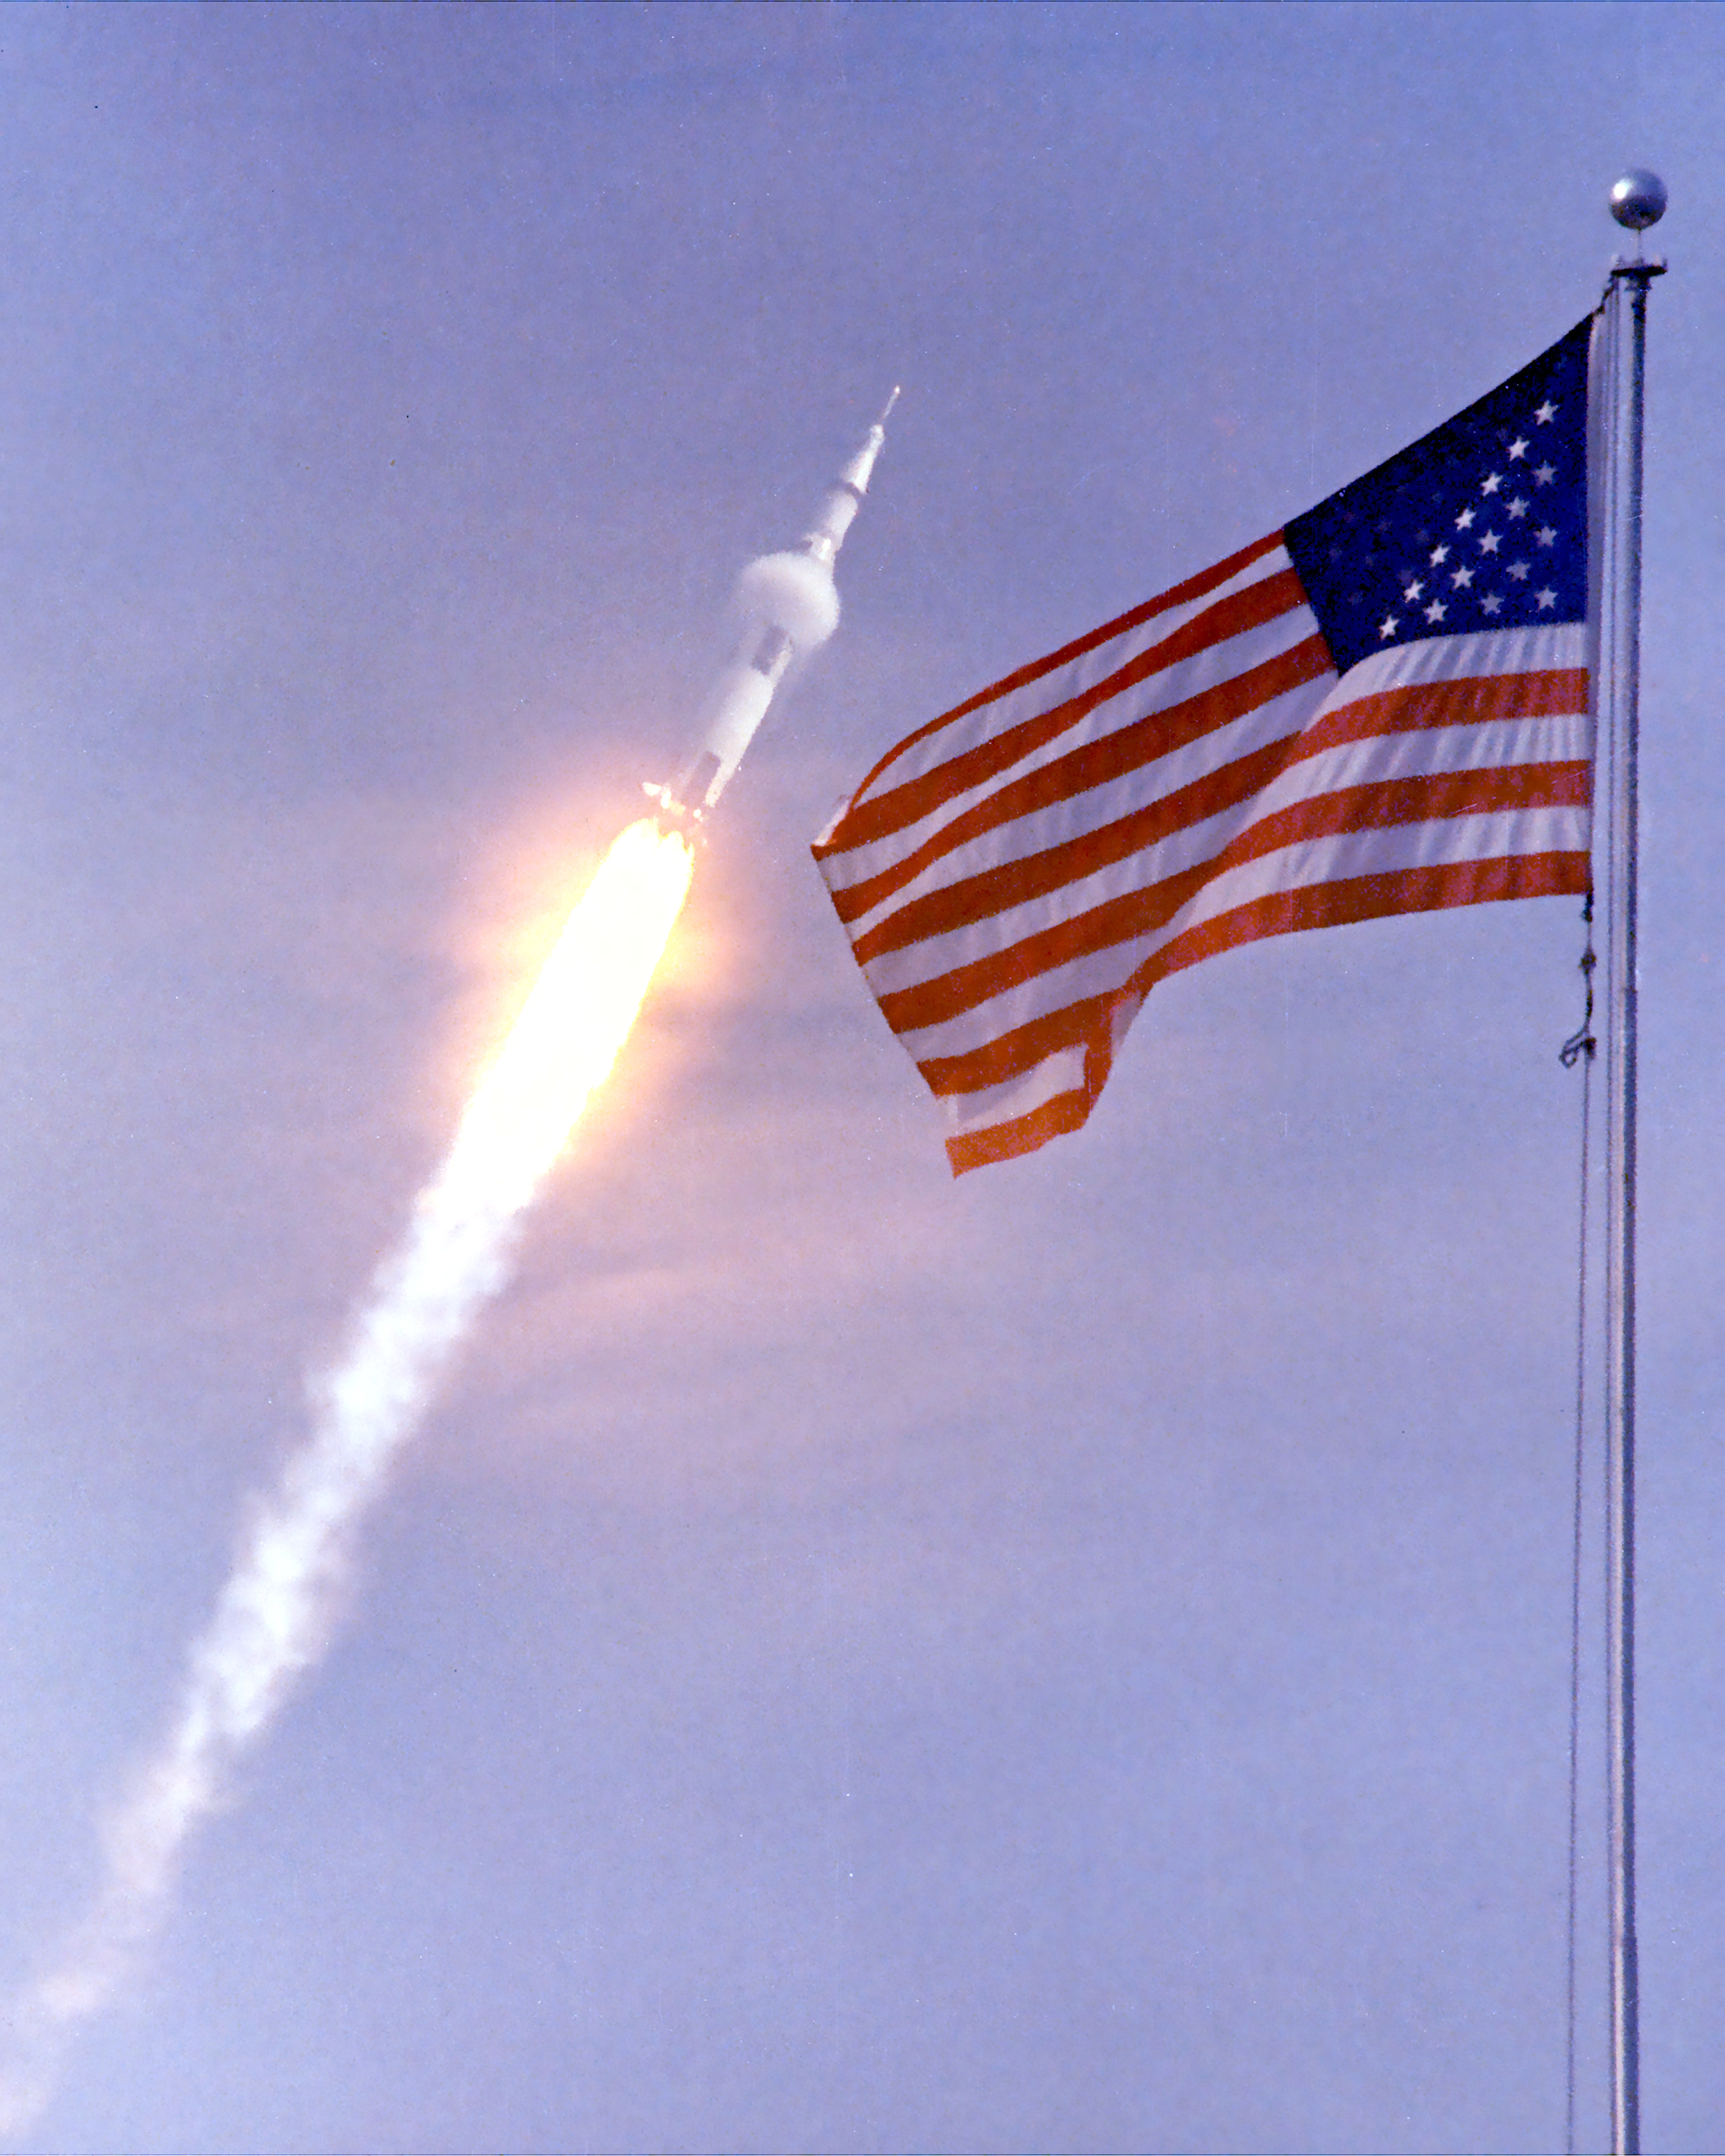
\includegraphics[width=0.92\textwidth]{images/saturn_v.jpg}
\captionof{figure}{Apollo 11 Saturn V launching on July 16, 1969. The rocket expels $13\,000\ \mathrm{kg\cdot s^{-1}}$ of hot combustion gas at $u_e \approx 2500\ \mathrm{m\cdot s^{-1}}$, generating $34\ \mathrm{MN}$ of thrust.}
\label{fig:saturn_v}
\end{minipage}\hfill
\begin{minipage}{0.48\textwidth}
\centering
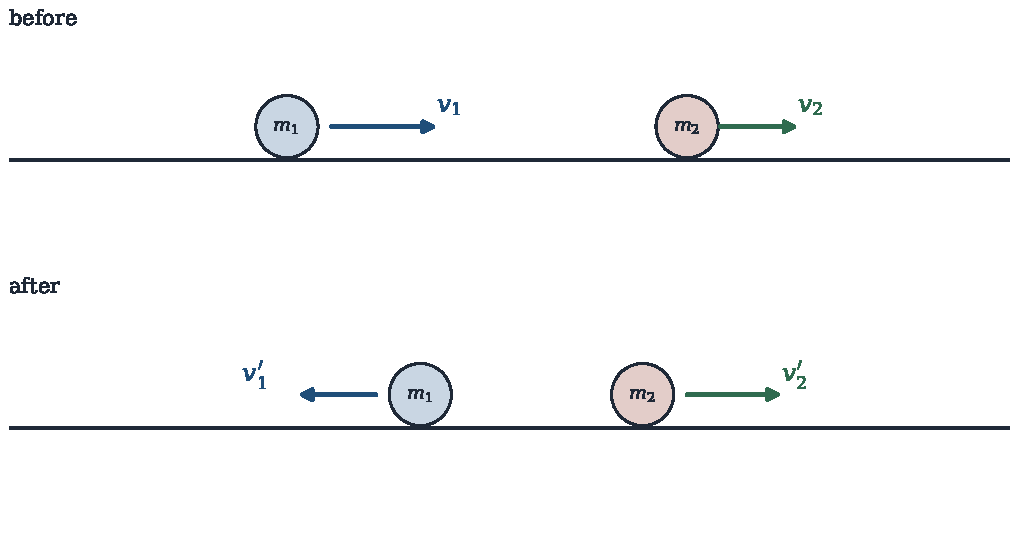
\includegraphics[width=0.92\textwidth]{figures/21_collision.pdf}
\captionof{figure}{Collision kinematics between two particles in the Laboratory frame (left) and the Center-of-Mass frame (right).}
\label{fig:collision}
\end{minipage}
\end{figure}

Consider a rocket of mass $m(t)$ moving at velocity $\vec{v}(t)$ at time $t$. During interval $\dd t$, the rocket ejects propellant mass $\dd m_e = -\dd m > 0$ backward with exit velocity $\vec{v}_e$ in the inertial frame.
The relative exhaust velocity with respect to the rocket is:
\begin{equation}
\vec{u}_e \eqdef \vec{v}_e - \vec{v}.
\end{equation}
The total momentum of the closed system (rocket + ejected parcel) at time $t$ is $\vec{P}(t) = m\vec{v}$.
At time $t + \dd t$, the rocket has mass $m + \dd m$ and velocity $\vec{v} + \dd\vec{v}$, while the ejected parcel has mass $-\dd m$ and velocity $\vec{v}_e = \vec{v} + \vec{u}_e$:
\[
\vec{P}(t + \dd t) = (m + \dd m)(\vec{v} + \dd\vec{v}) + (-\dd m)(\vec{v} + \vec{u}_e) = m\vec{v} + m\,\dd\vec{v} - \dd m\,\vec{u}_e + \mathcal{O}(\dd t^2).
\]
The net change in momentum is $\dd\vec{P} = m\,\dd\vec{v} - \dd m\,\vec{u}_e = \vec{F}_{\text{ext}}\,\dd t$.

\begin{lawbox}{Meshchersky's Rocket Dynamic Equation (1897)}
The instantaneous acceleration of a variable-mass vehicle is governed by:
\begin{equation}
m(t) \frac{\dd\vec{v}}{\dd t} = \vec{F}_{\text{ext}} + \frac{\dd m}{\dd t} \vec{u}_e = \vec{F}_{\text{ext}} + \vec{T}_{\text{thrust}},
\end{equation}
where the \textbf{rocket thrust} $\vec{T}_{\text{thrust}}$ is:
\begin{equation}
\vec{T}_{\text{thrust}} \eqdef \frac{\dd m}{\dd t} \vec{u}_e = \mu \norm{\vec{u}_e} \vec{u}_{\text{thrust}}, \qquad \mu = -\frac{\dd m}{\dd t} > 0.
\end{equation}
\end{lawbox}

\begin{historicalbox}{Konstantin Tsiolkovsky: Father of Astronautics}
\begin{minipage}{0.28\textwidth}
\centering
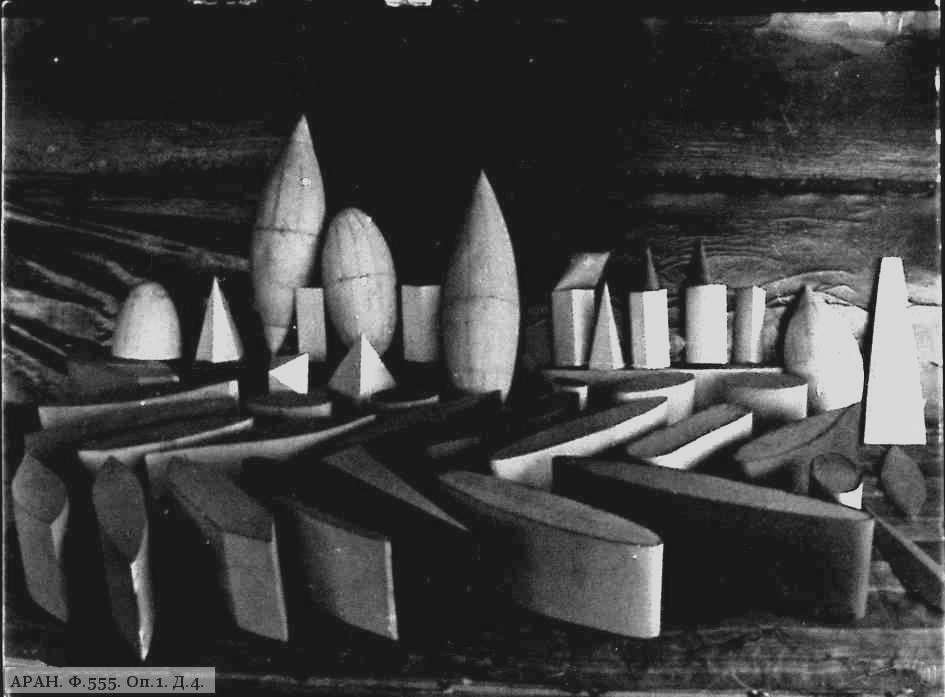
\includegraphics[width=0.92\textwidth]{images/tsiolkovsky.jpg}
\captionof{figure}{Konstantin Tsiolkovsky (1857--1935), Soviet pioneer of rocket science.}
\end{minipage}\hfill
\begin{minipage}{0.68\textwidth}
Working in near-total isolation as a deaf schoolteacher in the provincial Russian town of Kaluga, Konstantin Eduardovich Tsiolkovsky published his landmark paper in 1903: \emph{Exploration of Cosmic Space by Means of Reaction Devices}.

Tsiolkovsky mathematically proved that black gunpowder rockets could never escape Earth's gravity and proposed liquid-fuel engines running on liquid hydrogen and liquid oxygen. He invented multi-stage rocket trains, gyroscopic attitude stabilization, and closed-loop ecological life support, declaring: ``Earth is the cradle of humanity, but one cannot live in a cradle forever.''
\end{minipage}
\end{historicalbox}

\subsection{The Tsiolkovsky Rocket Equation}

In deep space where external forces vanish ($\vec{F}_{\text{ext}} = \vzero$), the 1D motion with propellant exhausted backward at speed $u_e$ satisfies:
\[
m\,\dd v = -u_e\,\dd m \implies \dd v = -u_e \frac{\dd m}{m}.
\]
Integrating from initial wet launch mass $m_0$ to final dry burnout mass $m_f$:
\[
\Delta v = \int_{m_0}^{m_f} -u_e \frac{\dd m}{m} = u_e \ln\left(\frac{m_0}{m_f}\right).
\]

\begin{lawbox}{The Tsiolkovsky Rocket Equation}
The characteristic burnout velocity increment $\Delta v$ achievable by a rocket in field-free space is:
\begin{equation}
\Delta v = u_e \ln\left(\frac{m_0}{m_f}\right) = g_0 I_{\text{sp}} \ln\left( \frac{m_0}{m_f} \right),
\end{equation}
where $I_{\text{sp}} \eqdef u_e/g_0$ is the engine \textbf{specific impulse} in seconds (with standard gravity $g_0 = 9.80665\ \mathrm{m\cdot s^{-2}}$).
In a uniform vertical gravitational field $\vec{g} = -g\,\khat$, vertical launch velocity is degraded by \textbf{gravity losses}:
\begin{equation}
v(t) = u_e \ln\left( \frac{m_0}{m(t)} \right) - g t.
\end{equation}
\end{lawbox}

\section{Collision Dynamics and Scattering Kinematics}

\begin{definitionbox}{Coefficient of Restitution (Newton, 1687)}
For a one-dimensional collision along the line of centers between particle 1 and particle 2, the \textbf{coefficient of restitution} $e$ is defined as the ratio of separation speed to approach speed:
\begin{equation}
e \eqdef \frac{|v_2' - v_1'|}{|v_1 - v_2|} = -\frac{v_2' - v_1'}{v_2 - v_1} \in [0, 1].
\end{equation}
\begin{itemize}[leftmargin=1.5em,itemsep=3pt]
  \item \textbf{Perfect Elastic Collision ($e = 1$):} Total kinetic energy is strictly conserved: $\Delta E_k = E_k' - E_k = 0$.
  \item \textbf{Partially Inelastic Collision ($0 < e < 1$):} Momentum is conserved, but kinetic energy is partially converted into internal deformation and heat: $\Delta E_k < 0$.
  \item \textbf{Perfect Inelastic (Plastic) Collision ($e = 0$):} The two bodies coalesce and move with a single common velocity $v_1' = v_2' = v_G$. The energy dissipation is maximized:
  \begin{equation}
  |\Delta E_k|_{\max} = \frac{1}{2} \mu (v_1 - v_2)^2, \qquad \mu \eqdef \frac{m_1 m_2}{m_1 + m_2}.
  \end{equation}
\end{itemize}
\end{definitionbox}

\section{Comprehensive Worked Examples}

\begin{workedexample}{Multi-Stage Rocket to Low Earth Orbit}
A spacecraft requires a total mission delta-v $\Delta v_{\text{req}} = 9200\ \mathrm{m\cdot s^{-1}}$ to reach Low Earth Orbit (including gravity and atmospheric drag losses). The rocket engines achieve an exhaust velocity $u_e = 3100\ \mathrm{m\cdot s^{-1}}$ ($I_{\text{sp}} \approx 316\ \mathrm{s}$).
\begin{enumerate}[leftmargin=1.4em,itemsep=3pt]
  \item Show that a single-stage rocket (SSTO) would require a structural-to-propellant mass ratio that is virtually impossible with modern aerospace alloys.
  \item Consider a two-stage rocket where each stage has identical exhaust velocity $u_e = 3100\ \mathrm{m\cdot s^{-1}}$ and provides half of the total velocity increment ($\Delta v_1 = \Delta v_2 = 4600\ \mathrm{m\cdot s^{-1}}$). Calculate the required mass ratio $m_{0i}/m_{fi}$ for each stage.
\end{enumerate}

\paragraph{Solution.}
\textbf{1. Single-Stage-to-Orbit (SSTO) Impossibility:}\\
Applying Tsiolkovsky's equation for a single stage:
\[
\Delta v = u_e \ln\left(\frac{m_0}{m_f}\right) \implies \frac{m_0}{m_f} = e^{\Delta v / u_e} = e^{9200 / 3100} = e^{2.9677} \approx 19.45.
\]
The final mass $m_f = m_{\text{structure}} + m_{\text{payload}}$ represents only:
\[
\frac{m_f}{m_0} = \frac{1}{19.45} \approx 0.0514 = 5.14\%.
\]
The propellant alone must constitute $94.86\%$ of the total launch mass. Because empty cryogenic tanks, rocket engines, turbopumps, avionics, and thermal insulation typically consume at least $6\text{--}8\%$ of dry structural mass, a single-stage chemical rocket cannot carry any useful payload to orbit.

\textbf{2. Two-Stage Rocket Staging Optimization:}\\
For each of the two stages:
\[
\Delta v_1 = \Delta v_2 = 4600\ \mathrm{m\cdot s^{-1}}.
\]
The required mass ratio for each stage is:
\[
\left(\frac{m_0}{m_f}\right)_1 = \left(\frac{m_0}{m_f}\right)_2 = e^{\Delta v_i / u_e} = e^{4600 / 3100} = e^{1.4839} \approx 4.41.
\]
The dry mass fraction for each individual stage is:
\[
\frac{m_{fi}}{m_{0i}} = \frac{1}{4.41} \approx 0.2268 = 22.7\%.
\]
Propellant constitutes only $77.3\%$ of each stage's mass! Dropping the empty first-stage tanks and heavy booster engines into the ocean eliminates the dead structural weight, allowing the second stage to ignite at high altitude and comfortably deliver several tons of scientific payload into orbit.
\end{workedexample}

\begin{workedexample}{Neutron Moderation and Energy Transfer in Nuclear Fission}
In a nuclear fission reactor, fission releases fast neutrons with kinetic energy $E_0 \approx 2.0\ \mathrm{MeV}$. To induce further fission in Uranium-235, these neutrons must be slowed down to thermal energies ($E_{\text{th}} \approx 0.025\ \mathrm{eV}$) through elastic collisions with stationary moderator nuclei of mass $M = A\,m_n$.
\begin{enumerate}[leftmargin=1.4em,itemsep=3pt]
  \item Derive the ratio of final to initial kinetic energy $E'/E_0$ for a head-on elastic collision.
  \item Compute the fractional energy loss $\xi \eqdef (E_0 - E')/E_0$ for:
  \begin{itemize}[leftmargin=1.2em]
    \item Ordinary Hydrogen ($A = 1$, light water $\mathrm{H_2O}$),
    \item Deuterium ($A = 2$, heavy water $\mathrm{D_2O}$),
    \item Carbon ($A = 12$, graphite),
    \item Uranium ($A = 238$).
  \end{itemize}
  \item Explain why light elements are uniquely suited as nuclear moderators.
\end{enumerate}

\paragraph{Solution.}
\textbf{1. Head-On Elastic Collision Kinematics:}\\
Let $m_n$ be the neutron mass and $M = A\,m_n$ be the target nucleus mass. In a head-on elastic collision with a stationary target ($v_2 = 0$):
\begin{align*}
m_n v_0 &= m_n v_1' + A m_n v_2', \\
\frac{1}{2}m_n v_0^2 &= \frac{1}{2}m_n (v_1')^2 + \frac{1}{2}A m_n (v_2')^2.
\end{align*}
Using Newton's restitution formula with $e = 1$:
\[
v_2' - v_1' = v_0 \implies v_2' = v_1' + v_0.
\]
Substituting $v_2'$ into the momentum equation:
\[
v_0 = v_1' + A(v_1' + v_0) = (A + 1)v_1' + A v_0 \implies v_1' = \left(\frac{1 - A}{1 + A}\right) v_0 = -\left(\frac{A - 1}{A + 1}\right) v_0.
\]
The final kinetic energy of the scattered neutron is:
\[
E' = \frac{1}{2}m_n (v_1')^2 = \left(\frac{A - 1}{A + 1}\right)^2 \left(\frac{1}{2}m_n v_0^2\right) \implies \frac{E'}{E_0} = \left(\frac{A - 1}{A + 1}\right)^2.
\]

\textbf{2. Fractional Energy Transferred:}\\
The fractional energy transferred to the target moderator nucleus is:
\[
\xi \eqdef \frac{E_0 - E'}{E_0} = 1 - \left(\frac{A - 1}{A + 1}\right)^2 = \frac{(A + 1)^2 - (A - 1)^2}{(A + 1)^2} = \frac{4A}{(A + 1)^2}.
\]
Evaluating $\xi$ for the different nuclei:
\begin{itemize}[leftmargin=1.5em,itemsep=3pt]
  \item \textbf{Hydrogen ($A = 1$):}
  \[
  \xi = \frac{4(1)}{(1 + 1)^2} = \frac{4}{4} = 1.000 \quad (\mathbf{100\%} \text{ energy transferred in a single collision!}).
  \]
  A fast neutron can lose its entire kinetic energy in a single billiard-ball collision with a proton of equal mass.
  \item \textbf{Deuterium ($A = 2$):}
  \[
  \xi = \frac{4(2)}{(2 + 1)^2} = \frac{8}{9} \approx 0.8889 = 88.9\%.
  \]
  \item \textbf{Carbon-12 ($A = 12$):}
  \[
  \xi = \frac{4(12)}{(12 + 1)^2} = \frac{48}{169} \approx 0.2840 = 28.4\%.
  \]
  \item \textbf{Uranium-238 ($A = 238$):}
  \[
  \xi = \frac{4(238)}{(238 + 1)^2} = \frac{952}{(239)^2} = \frac{952}{57\,121} \approx 0.0166 = 1.66\%.
  \]
\end{itemize}

\textbf{3. Physical Conclusion:}\\
Heavy elements like Uranium ($A = 238$) act as immovable brick walls: the light neutron bounces off elastically with virtually no energy loss ($98.3\%$ retained). Only light elements whose nuclear mass matches the neutron ($A \approx 1\text{--}2$) can absorb large fractions of kinetic energy per collision, allowing thermalization in just 18 to 25 collisions in water.
\end{workedexample}

\begin{workedexample}{Two-Dimensional Oblique Elastic Collision of Equal Masses}
A billiard ball $M_1$ of mass $m$ moving with speed $v_0$ along the $x$-axis collides elastically with an identical billiard ball $M_2$ of mass $m$ initially at rest. The collision is oblique (off-center).
\begin{enumerate}[leftmargin=1.4em,itemsep=3pt]
  \item Prove from vector conservation laws that the trajectories of the two balls after collision are \textbf{mutually perpendicular} ($90^\circ$ scattering angle), provided the collision is not head-on.
  \item If ball 1 is deflected by an angle $\theta_1 = 30^\circ$ relative to its initial incident direction, determine the deflection angle $\theta_2$ of ball 2, and the post-collision speeds $v_1'$ and $v_2'$.
\end{enumerate}

\paragraph{Solution.}
\textbf{1. Vector Proof of Orthogonality:}\\
Linear momentum conservation for two equal masses $m_1 = m_2 = m$ yields:
\[
m\vec{v}_0 = m\vec{v}_1' + m\vec{v}_2' \implies \vec{v}_0 = \vec{v}_1' + \vec{v}_2'.
\]
Because the collision is purely elastic, total kinetic energy is conserved:
\[
\frac{1}{2}m v_0^2 = \frac{1}{2}m (v_1')^2 + \frac{1}{2}m (v_2')^2 \implies v_0^2 = (v_1')^2 + (v_2')^2.
\]
Now take the scalar self-product (magnitude squared) of the momentum vector equation:
\[
v_0^2 = \vec{v}_0 \cdot \vec{v}_0 = (\vec{v}_1' + \vec{v}_2') \cdot (\vec{v}_1' + \vec{v}_2') = (v_1')^2 + (v_2')^2 + 2 (\vec{v}_1' \cdot \vec{v}_2').
\]
Comparing the two equations:
\[
(v_1')^2 + (v_2')^2 + 2 (\vec{v}_1' \cdot \vec{v}_2') = (v_1')^2 + (v_2')^2 \implies 2 (\vec{v}_1' \cdot \vec{v}_2') = 0.
\]
Therefore:
\begin{equation}
\vec{v}_1' \cdot \vec{v}_2' = 0.
\end{equation}
Unless one of the post-collision speeds vanishes (which occurs only for a direct head-on collision where $v_1' = 0$ and $v_2' = v_0$), the scalar product vanishes if and only if the velocity vectors are strictly orthogonal:
\[
\cos(\theta_1 + \theta_2) = 0 \implies \theta_1 + \theta_2 = 90^\circ.
\]

\textbf{2. Angles and Speeds for $\theta_1 = 30^\circ$:}\\
Since the total divergence angle is $90^\circ$:
\[
\theta_2 = 90^\circ - \theta_1 = 90^\circ - 30^\circ = 60^\circ.
\]
Projecting the momentum equation $\vec{v}_0 = \vec{v}_1' + \vec{v}_2'$ along the incident axis ($x$) and perpendicular axis ($y$):
\begin{align*}
v_1' \cos 30^\circ + v_2' \cos 60^\circ &= v_0, \\
v_1' \sin 30^\circ - v_2' \sin 60^\circ &= 0 \implies v_1'\left(\frac{1}{2}\right) = v_2'\left(\frac{\sqrt{3}}{2}\right) \implies v_1' = \sqrt{3}\,v_2'.
\end{align*}
Substituting $v_1'$ into the $x$-equation:
\[
(\sqrt{3} v_2')\left(\frac{\sqrt{3}}{2}\right) + v_2'\left(\frac{1}{2}\right) = v_0 \implies \frac{3}{2}v_2' + \frac{1}{2}v_2' = 2v_2' = v_0.
\]
Thus:
\[
v_2' = \frac{1}{2} v_0 = 0.50\,v_0, \qquad v_1' = \frac{\sqrt{3}}{2} v_0 \approx 0.866\,v_0.
\]
Checking kinetic energy conservation:
\[
(v_1')^2 + (v_2')^2 = \left(\frac{\sqrt{3}}{2} v_0\right)^2 + \left(\frac{1}{2} v_0\right)^2 = \left(\frac{3}{4} + \frac{1}{4}\right)v_0^2 = v_0^2.
\]
Energy and momentum are verified in every detail.
\end{workedexample}
